\section{Logistic Regression}

\subsection{Recommended References}
\begin{frame}{Logistic Regression - Recommended References}
	\begin{vfilleditems}
		\item \textcite{gelman2013bayesian} - Chapter 16: Generalized linear models
		\item \textcite{mcelreath2020statistical}:
		\begin{vfilleditems}
			\item Chapter 10: Big Entropy and the Generalized Linear Model
			\item Chapter 11, Section 11.1: Binomialregression
		\end{vfilleditems}
		\item \textcite{gelman2020regression}:
		\begin{vfilleditems}
			\item Chapter 13: Logistic regression
			\item Chapter 14: Working with logistic regression
			\item Chapter 15, Section 15.3: Logistic-binomial model
			\item Chapter 15, Section 15.4: Probit regression
		\end{vfilleditems}
	\end{vfilleditems}
\end{frame}

\begin{frame}{Welcome to the Magical World of the Linear Generalized Models}
	Leaving the realm of the linear models,
	we start to adventure to the generalized linear models -- GLM.
	\vfill
	The first one is \textbf{logistic regression}.
	(also called Bernoulli regression or
	binomial regression).
\end{frame}

\subsection{Binary Data}
\begin{frame}{Binary Data\footnote{
			also known as dichotomous, dummy, indicator variable, etc.}
	}
	We use logistic regression when our dependent variable is \textbf{binary}.
	It only takes two distinct values,
	usually coded as $0$ and $1$.
\end{frame}

\subsection{What is Logistic Regression}
\begin{frame}{What is Logistic Regression}
	Logistic regression behaves exactly as a linear model:
	it makes a prediction by simply computing a weighted sum of the
	independent variables $\mathbf{X}$ using the estimated coefficients $\boldsymbol{\beta}$,
	along with a constant term $\alpha$.
	However, instead of outputting a continuous value $\mathbf{y}$,
	it returns the \textbf{logistic function} of this value:
	$$
		\text{logistic}(x) = \frac{1}{1 + e^{-x}}
	$$
\end{frame}


\subsubsection{Logistic Functions}

\begin{frame}{Logistic Function}
	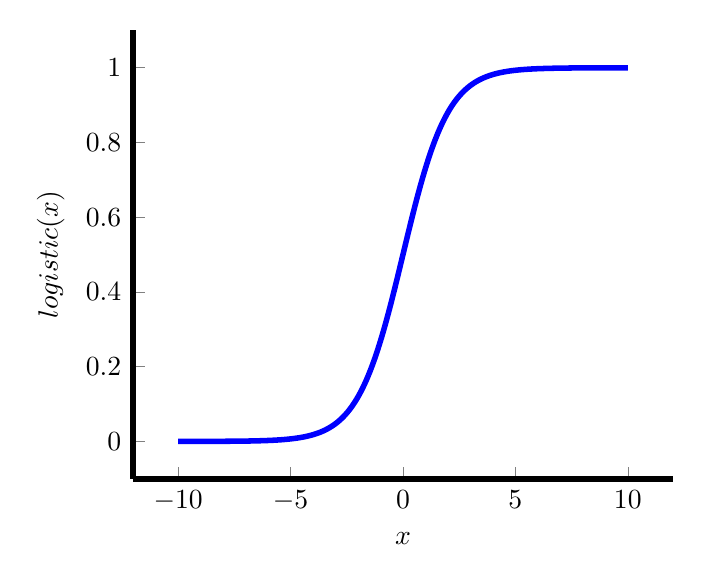
\begin{tikzpicture}
		\begin{axis}[every axis plot, line width=2pt,
				ylabel={$\text{logistic}(x)$},
				xlabel={$x$},
				domain=-10:10,samples=200,
				axis x line*=bottom, % no box around the plot, only x and y axis
				axis y line*=left % the * suppresses the arrow tips
			]

			\addplot [blue] (x,{1/(1+exp(-x))});
		\end{axis}
	\end{tikzpicture}
\end{frame}

\subsubsection{Probit Function}
\begin{frame}{Probit Function}
	We can also opt to choose to use the \textbf{probit function}
	(usually represented by the Greek letter $\Phi$)
	which is the CDF of a normal distribution:
	$$
		\Phi (x)= \frac {1}{\sqrt {2 \pi}}\int _{-\infty }^{x}e^{-t^{2}/2}\,dt
	$$
\end{frame}

\begin{frame}{Probit Function}
	\begin{tikzpicture}
		\begin{axis}[every axis plot, line width=2pt,
				ylabel={$\Phi(x)$},
				xlabel={$x$},
				domain=-10:10,samples=200,
				axis x line*=bottom, % no box around the plot, only x and y axis
				axis y line*=left % the * suppresses the arrow tips
			]

			\addplot [blue] {normcdf(0, 1)};
		\end{axis}
	\end{tikzpicture}
\end{frame}

\subsubsection{Logistic Function versus Probit Function}
\begin{frame}{Logistic Function versus Probit Function}
	\begin{tikzpicture}
		\begin{axis}[every axis plot, line width=1pt,
				ylabel={$f(x)$},
				xlabel={$x$},
				domain=-10:10,samples=200,
				axis x line*=bottom, % no box around the plot, only x and y axis
				axis y line*=left % the * suppresses the arrow tips
			]
			\addplot [blue] (x,{1/(1+exp(-x))});
			\addlegendentry{logistic}
			\addplot [red] {normcdf(0, 1)};
			\addlegendentry{probit}
		\end{axis}
	\end{tikzpicture}
\end{frame}

\subsection{Comparison with Linear Regression}
\begin{frame}{Comparison with Linear Regression}
	Linear regression follows the following mathematical expression:
	\small
	$$
		\text{linear} = \alpha + \beta_1 x_1 + \beta_2 x_2 + \dots + \beta_k x_k
	$$
	\begin{vfilleditems}
		\item \small $\alpha$ -- intercept.
		\item \small $\boldsymbol{\beta} = \beta_1, \beta_2, \dots, \beta_k$ -- independent variables' $x_1, x_2, \dots, x_k$ coefficients.
		\item \small $k$ -- number of independent variables.
	\end{vfilleditems}
	If you implement a small mathematical transformation,
	you'll have \textbf{logistic regression}:
	\begin{vfilleditems}
		\item \small $\hat{p} = \text{logistic}(\text{linear}) = \frac{1}{1 + e^{-\operatorname{linear}}}$ --
		probability of an observation taking value $1$.
		\item \small $\hat{y} = \begin{cases} 0 & \text { if } \hat{p} < 0.5 \\ 1 & \text { if } \hat{p} \geq 0.5 \end{cases}$ --
		$\mathbf{y}$'s predicted binary value.
	\end{vfilleditems}
\end{frame}

\subsection{Logistic Regression Specification}
\begin{frame}{Logistic Regression Specification}
	We can model logistic regression using two approaches:
	\begin{vfilleditems}
		\item \textbf{Bernoulli likelihood} --
		\textbf{binary} dependent variable \textbf{y} which results from a
		Bernoulli trial with some probability $p$
		\item \textbf{binomial likelihood} --
		\textbf{discrete and positive} dependent variable $\textbf{y}$
		which results from $k$ successes in independent Bernoulli
		trials.
	\end{vfilleditems}
\end{frame}

\subsubsection{Bernoulli Likelihood}
\begin{frame}{Bernoulli Likelihood}
	\small
	$$
		\begin{aligned}
			\mathbf{y}         & \sim \text{Bernoulli}\left( p\right)                                      \\
			p                  & \sim \text{logistic/logit}(\alpha +  \mathbf{X} \boldsymbol{\beta})       \\
			\alpha             & \sim \text{Normal}(\mu_\alpha, \sigma_\alpha)                             \\
			\boldsymbol{\beta} & \sim \text{Normal}(\mu_{\boldsymbol{\beta}}, \sigma_{\boldsymbol{\beta}})
		\end{aligned}
	$$
	where:
	\begin{vfilleditems}
		\item \small $\mathbf{y}$ - \textbf{dependent binary variable}.
		\item \small $p$ - probability of $\mathbf{y}$ taking value of $1$ --
		success in an independent Bernoulli trial.
		\item \small $\text{logistic/logit}$ -- logistic or logit function.
		\item \small $\alpha$ -- intercept (also called constant).
		\item \small $\boldsymbol{\beta}$ -- coefficient vector.
		\item \small $\mathbf{X}$ -- data matrix.
	\end{vfilleditems}
\end{frame}

\subsubsection{Binomial Likelihood}
\begin{frame}{Binomial Likelihood}
	\small
	$$
		\begin{aligned}
			\mathbf{y}         & \sim \text{Binomial}\left(n,  p\right)                                    \\
			p                  & \sim \text{logistic/probit}(\alpha +  \mathbf{X} \boldsymbol{\beta})      \\
			\alpha             & \sim \text{Normal}(\mu_\alpha, \sigma_\alpha)                             \\
			\boldsymbol{\beta} & \sim \text{Normal}(\mu_{\boldsymbol{\beta}}, \sigma_{\boldsymbol{\beta}})
		\end{aligned}
	$$
	where:
	\begin{vfilleditems}
		\item \small $\mathbf{y}$ - \textbf{discrete positive variable} -- $k$ successes of independent Bernoulli trials.
		\item \small $n$ - number of independent Bernoulli trials.
		\item \small $p$ - probability of $\mathbf{y}$ taking value of $1$ --
		success in an independent Bernoulli trial.
		\item \small $\text{logistic/logit}$ -- logistic or logit function.
		\item \small $\alpha$ -- intercept (also called constant).
		\item \small $\boldsymbol{\beta}$ -- coefficient vector.
		\item \small $\mathbf{X}$ -- data matrix.
	\end{vfilleditems}
\end{frame}

\subsubsection{Posterior Computation}
\begin{frame}{Posterior Computation}
	Our aim to is to \textbf{find the posterior distribution of the
		model's parameters of interest} ($\alpha$ and $\boldsymbol{\beta}$)
	by computing the full posterior distribution of:
	$$
		P(\boldsymbol{\theta} \mid \mathbf{y}) = P(\alpha, \boldsymbol{\beta} \mid \mathbf{y})
	$$
\end{frame}

\subsection{How to Interpret Coefficients}
\begin{frame}{How to Interpret Coefficients}
	If we revisit logistic transformation mathematical expression,
	we see that, in order to interpret coefficients $\boldsymbol{\beta}$,
	we need to perform a transformation.
	\vfill
	Specifically, we need to undo the logistic transformation.
	We are looking for its inverse function.
\end{frame}

\begin{frame}{Probability versus Odds}
	\small
	But before that, we need to discern between
	\textbf{probability and odds}\footnote{mathematically speaking.}.
	\begin{vfilleditems}
		\item \small \textbf{Probability}: a real number between $0$ and $1$
		that represents the certainty that an event will occur,
		either by long-term frequencies (frequentist approach) or
		degrees of belief (Bayesian approach).
		\item \small \textbf{Odds}: a positive real number ($\mathbb{R}^+$)
		that also measures the certainty of an event happening.
		However this measure is not expressed as a probability
		(between $0$ and $1$),
		but as the \textbf{ratio between the number of results that
			generate our desired event and the number of results that
			\textit{do not} generate our desired event}:
		$$
			\text{odds} = \frac{p}{1-p}
		$$
		where $p$ is the probability.
	\end{vfilleditems}
\end{frame}

\begin{frame}{Probability versus Odds}
	$$
		\text{odds} = \frac{p}{1-p}
	$$
	where $p$ is the probability.
	\vfill
	\begin{vfilleditems}
		\item Odds with a value of $1$ is a neutral odds,
		similar to a fair coin: $p = \frac{1}{2}$
		\item Odds below $1$ decrease the probability of seeing a certain event.
		\item Odds over $1$ increase the probability of seeing a certain event.
	\end{vfilleditems}
\end{frame}

\begin{frame}{Logodds}
	If you revisit the logistic function, you'll se that the intercept $\alpha$
	and coefficients $\boldsymbol{\beta}$ are literally the \textbf{log of the odds}
	(logodds):
	$$
		\begin{aligned}
			p                  & = \text{logistic}(\alpha +  \mathbf{X} \boldsymbol{\beta} )                 \\
			p                  & = \text{logistic}(\alpha) + \text{logistic}( \mathbf{X} \boldsymbol{\beta}) \\
			p                  & = \frac{1}{1 + e^{(-\boldsymbol{\beta})}}                                   \\
			\boldsymbol{\beta} & = \log(\text{odds})
		\end{aligned}
	$$
\end{frame}

\begin{frame}{Logodds}
	Hence, the coefficients of a logistic regression are expressed in logodds,
	in which $0$ is the neutral element,
	and any number above or below it increases or decreases, respectively,
	the changes of obtaining a ``success'' in $\mathbf{y}$.
	To have a more intuitive interpretation (similar to the betting houses),
	we need to \textbf{convert the logodds into chances} by undoing the $\log function$.
	We need to perform an \textbf{exponentiation} of $\alpha$ and $\boldsymbol{\beta}$
	values:
	$$
		\begin{aligned}
			\text{odds}(\alpha)               & = e^\alpha               \\
			\text{odds}({\boldsymbol{\beta}}) & = e^{\boldsymbol{\beta}}
		\end{aligned}
	$$
\end{frame}
